\documentclass{VUMIFPSkursinis}
\usepackage{graphicx}
\graphicspath{ {img/} }
\usepackage{algorithmicx}
\usepackage{algorithm}
\usepackage{algpseudocode}
\usepackage{amsfonts}
\usepackage{amsmath}
\usepackage{bm}
\usepackage{color}
\usepackage{longtable}
\usepackage{hyperref}  % Nuorodų aktyvavimas
\usepackage{url}


% Titulinio aprašas
\university{Vilniaus universitetas}
\faculty{Matematikos ir informatikos fakultetas}
\department{Programų sistemų katedra}
\papertype{Kursinis darbas}
\title{Pakartotinis kodo panaudojimas pirminio kriptovaliutų platinimo (ICO) išmaniuosiuose kontraktuose}
\titleineng{Code review in initial coin offering (ICO) smart contracts}
\status{3 kurso 1 grupės studentė}
\author{Agnė Mačiukaitė}
\supervisor{lekt. Gediminas Rimša}
\date{Vilnius \\ \the\year}


\bibliography{library} 

\begin{document}
\maketitle

\tableofcontents


\sectionnonum{Įvadas} \label{ivadas}

Programinės įrangos pernaudojimas leidžia naudoti programas keliuose projektuose. Tai yra svarbi strategija programinei įrangai norint padidinti sistemos efektyvumą ir kokybę. Taikant pernaudojamumą programuotojai naudojasi jau įgyvendintu kodu, kurį keičia taip, kad jis atitiktų dabartinio projekto reikalavimus \cite {Ravichandran2003}. Viena iš būtinų sąlygų kuriant pernaudojamą programinę įranga yra supratimas skirtingų kontekstų, kuriuose pernaudojama programinė įranga galėtų būti naudojama ir kaip būtų valdomas jos pernaudojamumas. Tai padeda programinės įrangos kūrėjams nuspręsti ar programinė įranga atitinka reikalavimus ir gali būti kuriama, jei taip, tai ką reikia parametrizuoti ir kaip struktūrizuoti programinę įrangą, kad vėliau būtų galima ją pritaikyti skirtingiems kontekstams \cite{Kang1990}.

Pirminio kriptovaliuto platinimo (angl. initial coin offering, toliau ICO) metu įmonė parduoda specializuotus kripto-žetonus žadėdami, kad žetonai veiks kaip mainų priemonė gaunat paslaugas įmonės platformoje. Žetonų pardavimas kuria kapitalą pradiniam įmonės platformos kūrimui nors nėra įsipareigojimo dėl būsimos paslaugos kainos (žetonais ar kitaip) \cite{Catalini2018}. Satoshi Nakamoto išleidęs baltąjį popierių (angl. whitepaper) \cite{Nakamoto2008} įvykdė ICO  ir taip surinko finansavimą pirmąjam blockchain ir kriptovaliutai Bitcoin. Bitcoin - skaitmeniniai pinigai, kurių pavedimai vyksta internete naudojantis decentralizuota vieša duomenų baze - blockchain \cite{Swan2015}. Šiuo metu du populiariausi blockchain yra Ethereum ir Bitcoin \cite{Luu}. Ethereum be savo kriptovaliutos turi ir kitą svarbų funkcionalumą - išmaniuosius kontraktus - Turing complete programą, kuri leidžia rašyti decentralizuotas aplikacijas \cite{Buterin2014}. Solidity - populiariausia kalba naudojama rašyti išmaniesiems kontraktams \cite{Dannen}. Problema - išmaniųjų kontraktų technologijos yra pakankamai jaunos, dėl to pakartotonio kodo panaudojimo bazė dar tik formuojasi. ICO kontraktai yra tiražuojami kopijavimo su modifikacijos būdu.

Programinės įrangos produktų linija (angl. product line software engineering, toliau PLSE) naudojama įmonėse pakartojamumui susijusiuose programinės įrangos produktuose numatyti. PLSE suteikia bendrą architektūrą ir pernaudojamą kodą programinės įrangos kūrėjams \cite{Svahnberg}. Toks kūrimas susideda iš savybių išskyrimo ir jų įgyvendinimo produkte. Gerai išskirtos produkto ypatybės padeda sukurti lengvai pernaudojamą programą. Savybės turi būti atrinktos atsižvelginat į jų paplitimą bei kintamumą srityje \cite{Lee2015}. Naudojantis PLSE produkto kūrėjai gali fokusuotis produkto specifikacijoje, o ne bendrų savybėse \cite{Svahnberg}.

Savybių modeliavimas yra pagrindinis metodas atrinkti bei valdyti bendrąsias ir kintamas savybes produktų linijoje. Programinės įrangos šeimos gyvavimo pradžioje savybių modelis padeda išskirti pagrindines savybes, kurios gelbsti kuriant naują rinką ar  norint išlikti jau esamoje. Taip pat savybių modelis leidžia išskirti rizikingas savybes, nuspėti, kokia yra visos programos ar atskirų savybių kaina. Vėliau savybių modeliavimas padeda išskirti variacijos taškus programinės įrangos architektūroje \cite{Czarnecki2004}. Savybių modeliavimas yra populiariausias PLSE kūrime nuo pat pirmojo jo pristatymo \cite{Kang1990}. Taip yra todėl, nes savybės yra pakankamai abstraktus konseptas padedantis efektyviai bendrauti suinterasuotoms šalims. Savybių modeliavimas yra intuitivus ir efektyvus būdas žmonėms išreikšti savybių paplitimą ir kintamumą programinės įrangos šeimoje \cite{Kang2013}. 

Šio darbo tikslas - ištirti pirminio finansavimo kriptovaliutomis (ICO) išmaniuosius kontraktus, nustatyti, kokios savybės yra pastavios, o kokios - kintamos bei pasiūlyti būdus kodo pernaudojamumui didinti. 

Tikslui pasiekti išsikelti uždaviniai:
\begin{enumerate}
\item Apžvelgti savybių modeliavimą programinės įrangos produktų linijos sričiai 
\item Surinkti virš 100 išmaniųjų kontraktų skirtų ICO
\item Išskirti surinktų kontraktų savybes į pastovias ir kintančias
\item Pasiūlyti ICO išmaniuosius kontraktus pagal išrinktas savybes
\end{enumerate}

\section{Savybių modeliavimas}
Savybių modeliavime bendri ir kintami bruožai yra modeliuojami iš produkto savybių perspektyvos PLSE, kuri yra suinterestuotų šalių interesas. Originalus savybių modeliavimas - FODA (angl. Feature-Oriented Domain Analysis (FODA), toliau FODA) \cite{Kang1990} - paprastas modelis, kuris savybes skirsto pagal tai iš ko jos susideda bei pagal bendrumą ir specializaciją naudojant AND/OR  diagramas. Savybės yra suskirstytos į būtinas, alternatyvias ir pasirenkamas pagal bendrus ir kintamus bruožus \cite{Kang2013}.

\subsection{Savybė} \label{savybe}

Kelios tos pačios srities aplikacijos turi daug bendrų galimybių, bet taip pat kiekviena aplikacija turi ir savo išskirtinumų. Tos galimybės iš naudotojo perspektyvos yra savybės \cite{Kang1990}. Savybės yra pagrindinis produkto skiriamasis bruožas. Skirtingi srities analizės metodai terminą „savybė" apibūdina šiek tiek kitaip. FODA \cite{Kang1990} savybę apibūdina kaip pastebimą ir skiriamą sistemos charakteristiką, kuri yra matoma įvairioms suinteresuotoms šalims \cite{Lee2015}.

FODA fokusuojasi ties kliento perspektyva, tai yra ties paslaugomis, kurias teikia aplikacija ir aplinka, kurioje dirbama. Savybės yra sistemos atributai, kurie tiesiogiai paveikia naudotoją \cite{Kang1990}. Skirtumas tarp savybės ir konceptualios abstrakcijos (pvz.: funkcijos, objekto) yra tai, kad funkcijos ir objektai yra naudojami specifikuojant vidines sistemos detales. Kitaip, funkcijos ir objektai yra konceptualios abstrakcijos, kurios yra identifikuojamos iš vidinės sistemos pusės. Savybė - aiškiai matoma  pagal charakteristiką, kuri gali išskirti produktą iš kitų. Todėl savybių modeliavimas turi išskirti iš išorės matomas charakteristikas produktuose bendrumo ir kintamumo atžvilgiu, o ne apibūdinti visas produkto modeliavimo detales (pvz.: funkcinis, objektais orientuotas modeliavimas). Suprantant produkto bendrus ir kintamus bruožus galima sukurti pernaudojamas funkcijas ir objektus \cite{Lee2015}.

\subsection{Savybių modelis}

FODA \cite{Kang1990} autoriai apibrėžia savybių modelį, kaip modelį, kuris turi pavaizduoti standartines sistemos šeimos savybes srityje ir santykius tarp jų. Trumpiau - savybių modelis yra hierarchiškai išskirstytų savybių rinkinys. Santykiai tarp savybių modelyje yra kategorizuojami į:
\begin{itemize}
\item Ir - visos vaikinės savybės turi būti pasirinktos
\item Alternatyva - tik viena vaikinė savybė gali būti pasirinkta 
\item Ar - viena ar daugiau gali būti pasirinkta
\item Būtina - savybė yra privaloma
\item Pasirenkama - savybė gali būti pasirenkama
\end{itemize}

Savybių diagrama yra grafinė savybių modelio reprezentacija. Tai medis, kur primityvios savybės - lapai, pagrininės - mazgai (pav. \ref{img:fm_rules}). Bendros savybės tarp skirtingų produktų yra modeliuojamos kaip būtinos, kai skirtingos savybės tarp jų žymimos kaip alternatyvios ar pasirenkamos (ang. optional) \cite{Batory2005}. Bendros savybės atributai yra paveldimi pagal visą jos specifikaciją. Visos pasirenkamos ar alternetyvios savybės, kurios negali būti pasirinktos, kai yra bendra savybė pasirinkta turi būti pažymėtos kaip tarpusavyje nesuderinamos (angl. mutually exclusive with). Visos pasirenkamos ir alternatyvios savybės, kurios turi būti pasirinktos, kai bendra yra pasirinkta, turi būti pažymėtos kaip privalomos. Savybių modelio dokumentacija susideda iš stuktūrinės diagramos hierarchiškai suskaidančios savybes indentifikuojančias pasirenkamas ir alternatyves savybes, savybių apibūdinimo ir taisyklių kompozicijos savybėms \cite{Kang1990}. 

\begin{center}
    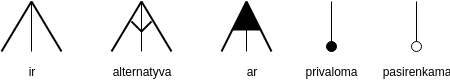
\includegraphics[scale=0.75]{img/feature_model_rules}
    \captionof{figure}{Savybių modelio žymėjimai \cite{Batory2005}}
    \label{img:fm_rules}
\end{center}

Pasirenkamos ir alternatyvios savybės negali būti atrinktos savavališkai. Įprastai jos parenkamos pagal galutinio naudotojo (kliento) tikslus ar interesus \cite{Kang1990}. Labai naudinga yra tai, kad savybė yra efektyvus komunikavimo būdas tarp suinteresuotų šalių. Dažnai klientai ir inžinieriai kalba apie produkto charakteristiką savybių pavidalu. Reikalavimai ir funkcijos yra apibūdinami kaip savybės kadangi jos yra aiškiai atpažįstamos abstrakcijos (plačiau \ref{savybe} Savybė) \cite{Lee2015}. Savybių modelis taip pat tarnauja kaip komunikacija tarp naudotojų ir kūrėjų. Naudotojui savybių modelis teikia informaciją, kokios yra savybės iš kurių gali rinktis ir kada. Kūrėjams savybių modelis identifikuoja, ką reiktų parametrizuoti kituose modeliuose bei programinės įrangos architektūroje ir kaip parametrizacija turi būti atlikta \cite{Kang1990}. Kitaip, savybių modelis gelbsti ne tik pernaudojamų komponentų kūrime, bet ir valdant produktų konfigūraciją srityje \cite{Lee2015}.

%Srities savybių modelis ir programinės įrangos architektūra turi būti apibrėžta aplink standartines savybes. Alternatyvios ir pasirenkamos savybės turi būti įtrauktos į modelį ir arcihtektūrą, bet visada turi būti parametrizuotos su atitinkamomis savybės, kad įsikyšimas į modelį ir architektūra būtų nesudėtingas \cite{Kang1990}. 


\subsection{Procesas ir gairės} \label{procesas}

Savybių analizė susideda iš reikalingų dokumentų surinkimo, savybių išskyrimo, savybių abstrakcijos ir identifikavimo modelyje, savybių apibrėžimo, modelio validacijos \cite{Kang1990}. Tačiau, prieš atliekant savybių modelį pirma turėtų būti išskirta sritis, kurios savybių alalizė bus atliekama \cite{Lee2015}. 

\subsubsection{Srities identifikavimas}

Srities identifikavimas prasideda nustantant sritį su kuria bus dirbama. Pasirinkus sritį turi būti nubrėžtos ribos ir santykiai tarp srities elementų ir kitų esybių esančių už srities ribų bei informacijos dalinimasis vieni tarp kitų. Srities modeliavimo tikslas yra nustatyti bendrus ir skirtingus konseptus ar charakteristikas sistemos kūrime \cite{Lee2015}.  

\subsubsection{Savybių identifikavimas} \label{identifikavimas}

Savybių identifikavimas susideda iš išskyrimo srities žinių gautų iš srities ekspertų ir kitų dokumentų tokių kaip knygos, nadotojo vadovo, projektavimo dokumentų ir jau parašytų programų \cite{Lee2015}. Aplikacijos savybes galima išskirti į keturias kategorijas:
\begin{itemize}
\item darbo aplinka, kurioje aplikacijos yra naudojamos
\item galimybės iš naudotojo perspektyvos 
\item srities technologija - kokiais reikalavimais remiantis sprendimas yra padaromas 
\item įgyvendinimo technika
\end{itemize}

%Metodas fokusuojasi ties savybėmis susijusiomis su aplikacijos galimybėmis. 

%Galimybių savybės dar gali būti suskirstytos į:
%\begin{itemize}
%\item funkcines
%\item operacines
%\item pateikimo (prezentacijps)
%\end{itemize}

%Funkcinės savybės yra servisai, kurie yra suteikti aplikacijos. Tokios savybės gali būti rastos naudotojo vadove bei reikalavimų dokumentacijoje. Operaicnės savybes - tos kurios susiję su aplikacijos operacijomis (taip pat iš vartotojo perspektyvos); tai yra, kaip naudotojas sčveikauja su aplikacija. Naudotojo vadivas yra geras tokių savybių šaltinis. Prezentacijos - tai kaip ir kokia informacija yra pateikama naudotojui. Tokia informacija randama naudotojo vadove ir reikalavimų specifikacijoje. 

Visos identifikuotos savybės turi būti pavadintos ir konfliktai susiję su vardais turi būti išspręsti. Savybių sinomimai taip pat turi būti įtraukti į srities terminologijos žodyną \cite{Kang1990}.

\subsubsection{Savybių abstrakcija, klasifikacija, modeliavimas}

Sekantis žingsnis identifikavus savybes turėtų būti hierarchinio modelio sukūrimas pagal savybių klasifikavimą, strūkturizavimą naudojant susideda iš santykį. Ar savybė yra būtina, alternatyvi, pasirenkama turi būti identifikuojama modelyje. Kiekviena savybė modelyje turi būti apibrėžta \cite{Kang1990}.

\subsubsection{Savybių modelio validacija}

Ar savybių modelis gerai reprezentuoja srities savybes turi būti validuota prieš srities ekspertus ir  jau egzituojančias aplikacijas. Srities ekspertai, kurie konsultavo analizės metu, neturi dalyvauti validacijoje. Taip pat bent viena aplikacija, kuri nebuvo naudota analizėje, turi būti panaudota, kad  būtų nustatytas modelio bendrumas ir pritaikomumas. Jei įmanoma validuojant turi būti panaudotas naujas aplikacijų rinkinys \cite{Kang1990}.
 


\section{Savybių modeliavimas ICO išmaniesiems kontraktams}

Buvo pasirinkta atlikti savybių modeliavimą remiantis procesu aprašytu \ref{procesas} skyriuje. Savybių modeliavimas buvo pradėtas nuo srities nusistatymo (plačiau \ref{sritis} Srities identifikavimas), tada buvo surinkta informacija reikalinga srities modelio sudarymui ir savybių išskyrimui bei atrinktos savybės (plačiau \ref{isskyrimas} Savybių identifikavimas), sekantis žingsnis buvo modelio sudarymas (plačiau \ref{modelis} Savybių modelis) ir jo validacija (plačiau \ref{validacija} Savybių modelio validacija).

\subsection{Srities identifikavimas} \label{sritis}

Šio savybių modeliavimo sritis - išmanieji kontraktai pirminiam kriptovaliutų platinimui. Kaip jau buvo minėta \ref{ivadas} įvade: „Išmaniųjų kontraktų technologijos yra pakankamai jaunos, dėl to pakartotinio kodo panaudojimo bazė dar tik formuojasi. ICO kontraktai yra tiražuojami kopijavimo su modifikacijos būdu." Todėl šiame savybių modeliavime bus apsirobojama tik ICO naudojamais kontraktais ir nebus analizuojami santykiai su kitais išmaniaisiais kontraktais ar sistemomis.


\subsection{Savybių identifikavimas} \label{isskyrimas}

Savybių modelio sukūrimui yra būtinas savybių identifikavimas. Remiantis \ref{identifikavimas} skyriuje aprašytu savybių identifikavimo būdais buvo pasirinktas jau parašytų programų (šiuo atveju išmaniųjų kontraktų) surinkimas, analizavimas ir savybių juose identifikavimas. Išmaniųjų kontraktų surinkimo procesas:
\begin{enumerate}
\item Iš Ethereum blockchain blokų naršyklės - etherscan.io, buvo atrinkti išmaniųjų kontraktų adresai ir nuorodos į juos platformoje
\item Parašytas interneto skaitytuvas (angl. web crawler) naudojantis Node.js karkasu
\item Visi surinktų išmaniųjų kontraktų kodai buvo surašyti į failus. Failo pavadinino struktūra: contract + identifikacijos numeris + .sol plėtinys
\end{enumerate}

Tokiu būdu buvo surinkta 128 pirminio kriptovaliutų platinimo išmanieji kontraktai. Savybės iš išmaniųjų kontraktų buvo išskirtos analizavimo būdu - pirmiausia atrinkta 21 išmanusis kontraktas, kuris neturi savybės - žetono sukūrimas ir disponavimas (priežastys šiam pasirinkimui yra pateiktos \ref{sritis} skyriuje). Išanalizavus atrinktus kontraktus buvo išskirtos savybės ir apibūdintos dalinai naudojantis forma pateikta FODA \cite{Kang1990}:

\begin{center}
    \begin{longtable}[H]{| p {4cm} | p{4cm} | p{4cm} | p{4cm} |}
    \hline
    Savybės pavadinimas  & Apibūdinimas & Susideda iš & Šaltiniai \endhead \hline
	
	Žetono kainos nustatymas skirtingomos pakopomis  & ICO metu žetonas gali turėti kelias kainas, skirtinga pakopa žetonų platinime - skirtinga kaina & lalal & contract2, contract23, contract43, contract46, contract55, contract62, contract85, contract120
 \\ 
	\hline
	
	ICO būsenos nustatymas & ICO gali turėti kelias būsenas, tokias kaip: neprasidėjo, prasidėjo, surinkta maksimali suma ir t.t. &  lalal & contract2, contract23, contract46, contract62, contract94, contract114, contract120, contract126 \\ 
	\hline
	
	
	Minimalaus investavimo kriterijus & Naudotojas turi būtinai ivestuoti sumą nemažensę nei minimalus investavimo kriterijus &  lalal & contract2, contract16, contract46, contract106  \\ 
	\hline
	
	ETH susigrąžinimo galimybė nepasiekus tikslo & Jei ICO nepasiekia nusistatyto minimalaus suinvestuotų pinigų ribos, tai visi investuoti pinigai yra grąžinami naudotojams &  lalal & contract2, contract23, contract46, contract62, contract85, contract94, contract96, contract120  \\ 
	\hline
	
	Žetonų atsiėmimas tik įvykus ICO & Įvykus ICO naudotojai gauna nusipirktus žetonus &  lalal & contract2, contract126 \\ 
	\hline
	
	Žetono ir fondo adresų nustatymas & Žetono ir fondo piniginių adresai gali būti nustatyti pakartotinai &  lalal & contract2, contract12, contract31, contract40,contract62, contract94, contract96, contract114, contract120  \\ 
	\hline
	
	Kainos už žetoną pakeitimas & Žetono kaina gali kisti neatsižvelgiant į pasikeičiančias pakopas &  lalal & contract2, contract40  \\ 
	\hline
	
	Kontrakto savininko nustatymas bei kai kurio funkcionalumo priskyrimas tik jam & Išmanusis kontraktas turi priviligijuotą adresą - kontrakto savininką, kuris turi daugiau funkcionalumo nei įprastas naudotojas &  lalal & contract2, contract12, contract13, contract16, contract23, contract31, contract43, contract46, contract62, contract72, contract85, contract86, contract94, contract106, contract114, contract116, contract120, contract126 \\ 
	\hline
	
	Galimybė sustabdyti ICO ir vėl paleisti iš naujo & ICO sustabdymo metu nebūtų galima nusipirkti žetonų &  lalal &  contract12, contract31\\ 
	\hline
	
	Galimybė pirkimo metu nustatyti kitą adresą kaip pirkėją & Naudotojas pirkdamas žetonus nustato adresą (pirkėją), kurį atstovauja &  lalal & contract12, contract31, contract62  \\ 
	\hline
	
	Pirkimas tik indentifikuotiems naudotojams & Pirkti žetonus gali tik anksčiau į kontraktą pridėti naudotojai &  lalal & contract12, contract16, contract31 \\ 
	\hline
	
	ICO sustabdymas ar galimybė keisti datą & ICO galima sustabdyti ar keisti jo pabaigos datą &  lalal & contract16, contract43, contract46, contract86, contract106  \\ 
	\hline
	
	Pelno pasiskirstymas tarp komandos ir kompanijos & Surinkta pinigų suma yra paskirtita ne tik kompanijai, bet ir komandai &  lalal &  contract23\\ 
	\hline
	
	ICO pradžios nustatymas  & ICO pradžios data gali būti keičiama &  lalal &  contract40, contract86, contract106, contract126 \\ 
	\hline
	
	Fondas atskirtas nuo kontrakto šeimininko & Išmaniojo kontrakto fondas ir savininkas yra dvi skirtingos piniginės &  lalal &  contract2, contract12, contract16, contract23, contract31, contract43, contract46, contract62, contract85, contract106, contract114, contract120, contract126\\ 
	\hline
	
	Maksimalaus galimo surinkti ETH keitimas & Galimybė papidinti ar sumažinti investicijų sumos skaičių &  lalal & contract43, contract86 \\ 
	\hline
	
	Nustatytas maksimalus galimas žetonų kiekis nupirktas per kartą & Naudotojas gali nusipirkti ne daugiau žetonų nei yra nustatyta &  lalal & contract43 \\ 
	\hline
	
	Nereikalingų žetonų išsitraukimas iš kontrakto  & Likusių žetonų nuo ICO susigrąžinimas &  lalal & contract13, contract62, contract94, contract114, contract120, contract126 \\ 
	\hline
	
	Žetonų išskyrimas komandai & Žetonų paskirstymas komandos nariams &  lalal &  contract62, contract72, contract94, contract114, contract120, contract126\\ 
	\hline


    \end{longtable}
    \captionof{table}{ICO išmaniųjų kontraktų savybės}

\end{center}



\subsection{Savybių modelis} \label{modelis}
\subsection{Savybių modelio validacija} \label{validacija}





\sectionnonum{Rezultatai}



\sectionnonum{Išvados}
Išvadose ir pasiūlymuose, nekartojant atskirų dalių apibendrinimų,
suformuluojamos svarbiausios darbo išvados, rekomendacijos bei pasiūlymai.



\printbibliography[heading=bibintoc] % Literatūros šaltiniai aprašomi
%bibliografija.bib faile. Šaltinių sąraše nurodoma panaudota literatūra,
%kitokie šaltiniai. Abėcėlės tvarka išdėstoma tik darbe panaudotų (cituotų,
%perfrazuotų ar bent paminėtų) mokslo leidinių, kitokių publikacijų
%bibliografiniai aprašai (šiuo punktu pasirūpina LaTeX). Aprašai pateikiami
% netransliteruoti.

\sectionnonum{Sąvokų apibrėžimai}
Turing complete - bet kuri sistema, kuri yra pakankamai galinga atpažinti visus galimus algoritmus \cite{Teller1994}. 

Interneto skaitytuvas (anlg. web crawler) - programa, kuri nuskaito puslapį ar kelis, nuskaito informacija juose ir grąžina rezultatą \cite{Thelwall2001}.

Node.js - vienos gijos Javascript serverio pusės karkasas \cite{Mccune}.


\sectionnonum{Santrumpos}
PLSE - programinės įrangos produktų linija (angl. product line software engineering)

ICO - pirminis kriptovaliutų platinimas (angl. initial coin offering)

FODA - Feature-Oriented Domain Analysis \cite{Kang1990}

%\appendix  % Priedai
% Prieduose gali būti pateikiama pagalbinė, ypač darbo autoriaus savarankiškai
% parengta, medžiaga. Savarankiški priedai gali būti pateikiami kompiuterio
% diskelyje ar kompaktiniame diske. Priedai taip pat vadinami ir numeruojami.
% Tekstas su priedais siejamas nuorodomis (pvz.: \ref{img:mlp}).
%

\end{document}
